\documentclass[border=2pt]{standalone}

% Drawing
\usepackage{tikz} 
\usepackage{tikz-3dplot}

% Tikz Library
\usetikzlibrary{angles, quotes}

% Style
\tikzset{>=latex}

% Define Color
\definecolor{amber}{rgb}{1.0, 0.5, 0}
\definecolor{darkmagenta}{rgb}{0.55, 0.0, 0.55}
\definecolor{bleudefrance}{rgb}{0.19, 0.55, 0.91}

% Notation
\usepackage{physics}

% Newcommand 
\newcommand{\midlabelline}[3]{
   \node (midlabel) at ($ (#1)!.5!(#2) $) {\huge #3};
   \draw[<-, very thick] (#1) --  (midlabel);
   \draw[->|, very thick] (midlabel) -- (#2);
}
\newcommand{\midlabellinee}[3]{
   \node (midlabel) at ($ (#1)!.5!(#2) $) {\huge #3};
   \draw[|<-, very thick] (#1) --  (midlabel);
   \draw[->|, very thick] (midlabel) -- (#2);
}

\newcommand{\midlabellineee}[3]{
   \node (midlabel) at ($ (#1)!.5!(#2) $) {\huge #3};
   \draw[very thick] (#1) --  (midlabel);
   \draw[very thick] (midlabel) -- (#2);
}

%Styles
%%Arrow in the Middle
\tikzset{midarrow/.style = {postaction=decorate, decoration={markings,mark=at position .52 with \arrow{stealth}}}}

% Define Length
\def\dy{0.45}

\begin{document}

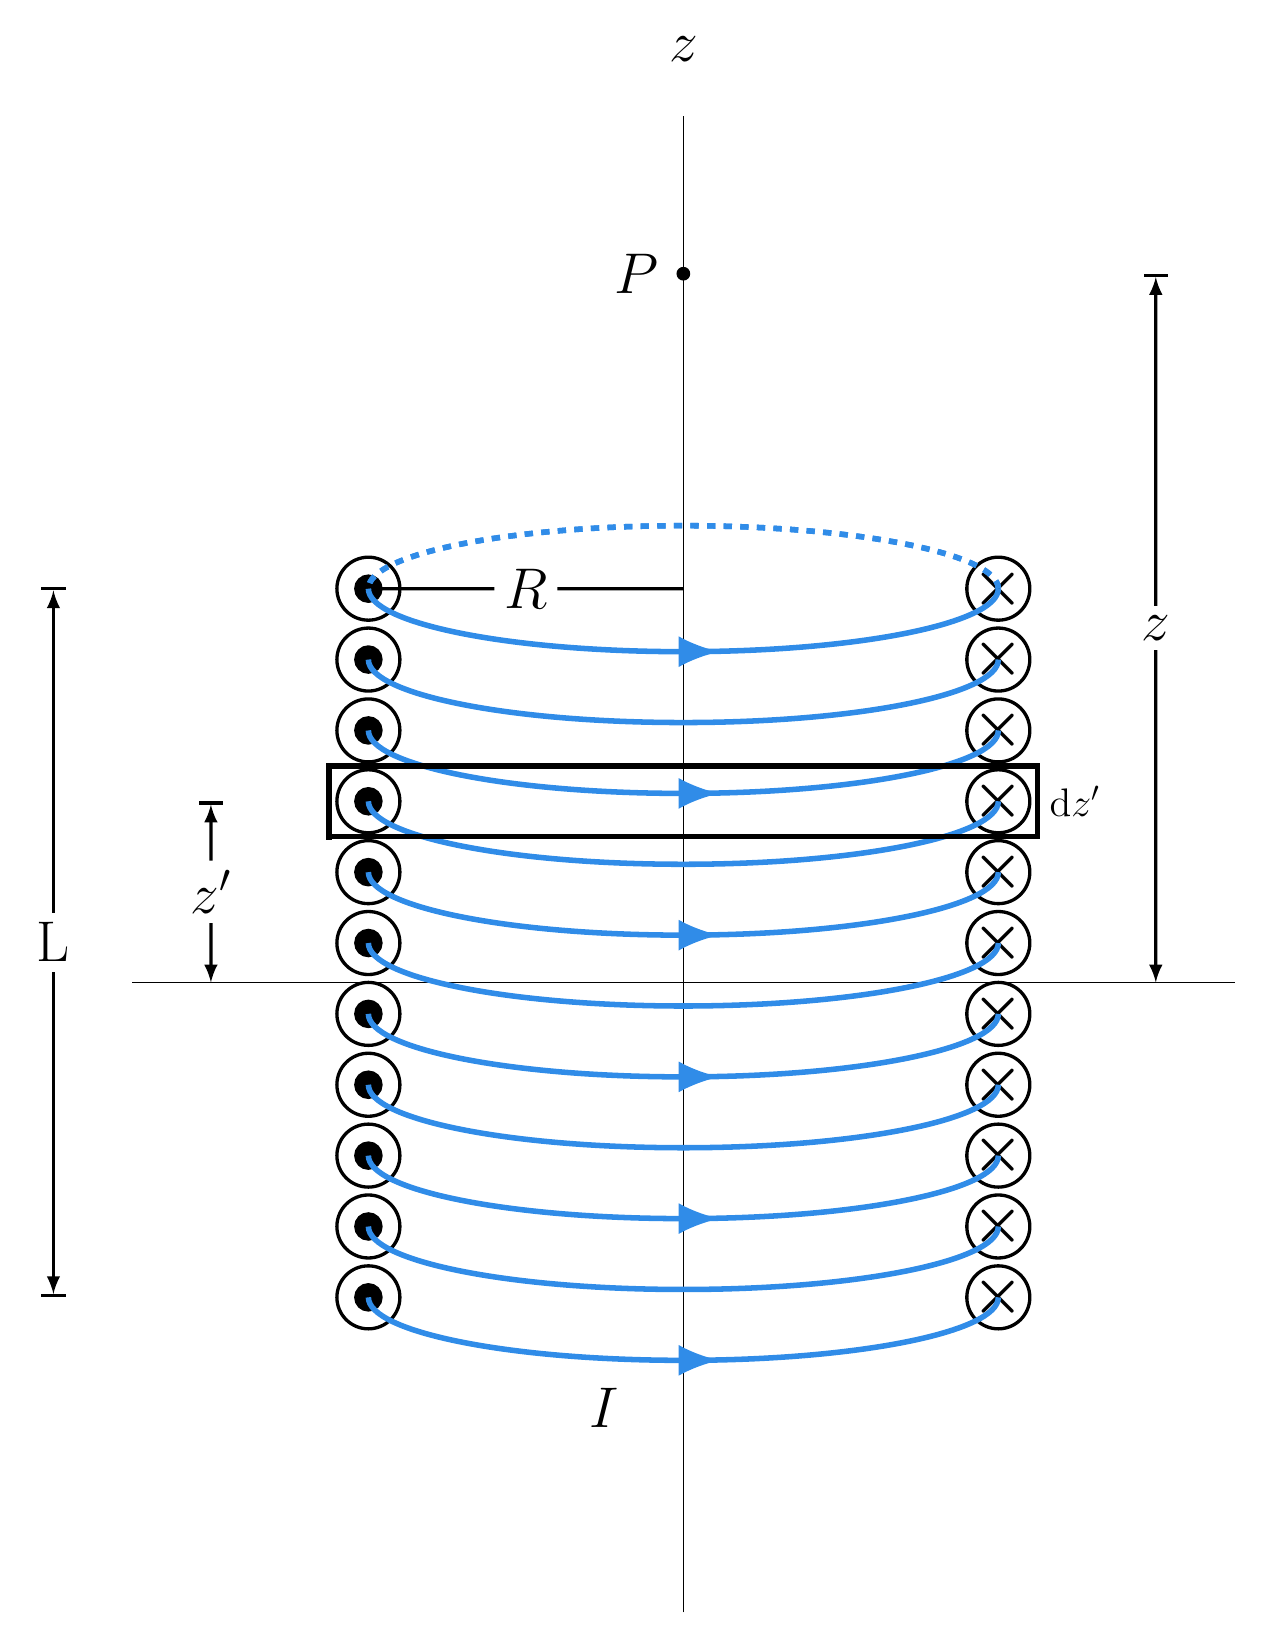
\begin{tikzpicture}[scale=2]
	% Grid
%	\draw[help lines] (0,0) grid (13,13);
	
	% Symbols of Field Direction
	%% Left
	\foreach \i in {0,1,2,...,10}
	{
		\draw[very thick] (4,9-\i*\dy) circle [radius=0.2];
		\filldraw[very thick] (4,9-\i*\dy) circle [radius=0.08];
	}
	%% Right
	\foreach \i in {0,1,2,...,10}
	{
		\draw[very thick] (8,9-\i*\dy) circle [radius=2mm];
		\node at (8,9-\i*\dy) {\huge$\cross$};
	}

	% Semi Circle Dashed
	\draw[dashed, bleudefrance, line width = 2] (8,9) arc (0:180: 2 and 0.4);
	
	% Axis
	\draw (2.5,6.5) -- (9.5,6.5);
	\draw (6,2.5) -- (6,12) node [above, pos = 1.03] {\huge$z$};
	
	% Label Distances
	\midlabellinee{2,4.5}{2,9.01}{L}
	\midlabelline{3,6.5}{3,7.65}{$z'$}
	\midlabelline{9,6.5}{9,11}{$z$}
	\midlabellineee{6,9}{4,9}{\huge$R$}
	
	% Semi Circles
	\foreach \i in {0,1,2,...,10}
	{
		\draw[bleudefrance, line width = 2] (4,9-\i*\dy) arc (180:360: 2 and 0.4);
	}
	
	\foreach \i in {0,1,2,...,5}
	{
		\draw[bleudefrance, line width = 4, ->] (6.05,8.6-2*\i*\dy) -- (6.230,8.6-2*\i*\dy);
	}
	%% Dashed
	\draw[dashed, bleudefrance, line width = 2] (8,9) arc (0:180: 2 and 0.4);

	% Point
	\filldraw (6,11) circle [radius=0.04];	
	\node at (5.7,11) {\huge$P$};
	
	% Rectangle with Label
	\draw[line width = 2] (3.75,7.425) -- ++(4.5,0) -- ++(0,0.45) node [midway, right] {\Large$\mathrm{d}z'$} -- ++(-4.5,0) -- ++(0,-0.468);
	
	% Node
	\node at (5.5,3.8) {\huge$I$};
\end{tikzpicture}
	
\end{document}